\documentclass[journal,twoside,letterpaper]{IEEEtran}
%\documentclass[draftcls]{IEEEtran}

\usepackage[english]{babel} 
\usepackage{cite}
\usepackage[pdftex]{graphicx}
\graphicspath{{img/}}
\usepackage[cmex10]{amsmath}
\usepackage{amssymb}
\interdisplaylinepenalty=2500
\usepackage{array}
\usepackage{mdwmath}
\usepackage{mdwtab}
\usepackage{eqparbox}
\hyphenation{op-ti-cal net-works se-mi-con-duc-tor har-mo-nics har-mo-nic}
\renewcommand{\vec}[1]{\mathbf{#1}}
\newcommand{\mat}[1]{\left[#1\right]}
\newcommand{\tensor}[1]{\bar{\bar{#1}}}
\DeclareMathOperator{\diag}{diag}
\usepackage{color}

\usepackage{stfloats}

\begin{document}

\title{Harmonic Balance Finite Element Analysis of Microwave Ferroelectric Devices}
\author{****
%Laurent~Ntibarikure,~\IEEEmembership{Member,~IEEE}, Stefano~Selleri,~\IEEEmembership{Senior Member,~IEEE}, Giuseppe~Pelosi,~\IEEEmembership{Fellow,~IEEE}
%\thanks{Corresponding e-mail: stefano.selleri@unifi.it}
}

\markboth{Microwave and Optical Tecnology Letters, VOL. X, NO. X, Month XXXX}{Microwave and Optical Technology letters, VOL. X, NO. X, Month XXXX}

\maketitle

\begin{abstract}
A full-wave finite element approach to the computation of higher order harmonics generated in ferroelectric materials is here presented. The harmonic vector wave equation finite elements formulation is extended into a multi-harmonic form, where non-linear material properties provides the coupling coefficients between the harmonics. Based on reported third order spurious signals measurements, a Barium-Strontium-Titanate thin-film coplanar transmission line model is employed to evaluate the validity of the proposed method.
\end{abstract}

\begin{IEEEkeywords}
Barium-Strontium-Titanate (BST), coplanar waveguide (CPW), harmonic balance, finite element method, ferroelectric, nonlinear modeling
\end{IEEEkeywords}

\IEEEpeerreviewmaketitle

\section{Introduction}

\IEEEPARstart{F}{erroelectric} materials exhibit unique opportunities to facilitate the reconfiguration of microwave devices and their performance metrics. In their most conceptual form, they impart the ability to alter the dielectric and conductive material properties both locally and across an entire device.

The use of ferroelectric materials in the design of varactors, switches, tunable phase shifters and reconfigurable antennas has been reported in recent years \cite{Kong2012, wang2005high, Sazegar2011, li2015cpw, Mansour2016, He2019}. In particular, Barium-Strontium-Titanate (BST) oxides, a well-researched group of ceramic materials, have been extensively employed in frequency agile microwave devices, mainly for their increased fabrication speed at a lower cost \cite{furlan2015influence}.

Among the available electromagnetic full-wave analysis methods of nonlinear microwave devices, the finite differences in time domain is known to provide reliable predictions but often results to be computationally prohibitive, especially for thin film planar devices \cite{furlan2015influence}. Both space and time domains must be carefully limited in order to decrease simulation times \cite{caudle2013three}.

When a finite set of frequencies is sufficient to characterize a device, a time-harmonic finite element (FE) method might be used. However, harmonic distortion due to material non-linearities cannot accurately be modeled with a single harmonic approach. Physically engendered high-order harmonics and their coupling behavior might be included by using the harmonic balance finite element (HBFE) method \cite{Yamada1989,Gyselinck2002, Copeland2010}, which is known to provide a fast and accurate solution for magneto-quasi-static problems. This method may allow to predict higher order spurious signals, known to dramatically reduce the large signal performances of BST based devices\cite{price2012temperature}.

This paper extends the methodology presented in \cite{Ntibarikure2012}, in which a \mbox{2-D} HBFE analysis of an H-plane waveguide filter was reported, to the \mbox{3-D} case of arbitrarily shaped passive nonlinear microwave devices. First, the conventional finite elements formulation is presented, including the numerical solution of eigenmodes at port boundaries. Then, the harmonic balance is introduced upon extending the number of harmonics and defining their coupling properties. Finally, a modeled transmission line including nonlinear dielectrics is analysed, and the results are compared with reported measurements.

%%%%%%%%%%%%%%%%%%%%%%%%%%%%%%%%%%%%%%%%%%%%%%%%%%%%%%%%%%%%%%%%%%%%%%%%%%%%%%%%
\section{Formulation}
\subsection{Conventional Time-Harmonic Finite Elements}

\label{sec:FE}
\begin{figure}[t!]
\centering
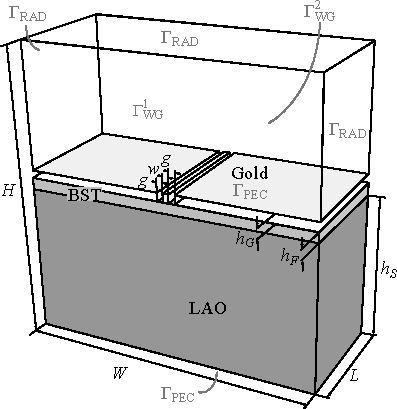
\includegraphics[width=8cm]{CPW}
\caption{Coplanar waveguide as the domain $\Omega$ of analysis and relative boundaries: $\Gamma_\text{PEC}$ for the perfect electric conductor on ground plane and golden metalisations, $\Gamma_\text{RAD}$ for the absorbing boundary conditions, and wave ports boundary conditions on $\Gamma_\text{WG}^1$ and $\Gamma_\text{WG}^2$. The center conductor strip and gaps aside are $w = g = 20~{\mu}$m, and the thickness is $h_G = 0.3~{\mu}$m. The thickness of the  BST film and the LAO substrate are, respectively, $h_F = 400$~nm and $h_S = 500~{\mu}$m. Dimensions of the box are $W = H = 1$~mm and $L=0.42$~mm.}
\label{fig:CPW}
\end{figure}

Let us consider, without loss of generality, the unshielded coplanar waveguide (CPW) of Fig. \ref{fig:CPW}, its domain $\Omega \subset \mathbb{R}^3$ with boundary $\Gamma \subset \mathbb{R}^2$.
%
The electric field $\vec{E}$ satisfies, within $\Omega$, the second-order wave equation \cite{Pelosi2009}
%
\begin{equation}
\label{eq:helmholtz}
\nabla \times \frac{1}{\mu_r} \nabla \times \vec{E} - {k}_0^2 {\varepsilon}_r \vec{E} = 0, \quad \text{in } \Omega
\end{equation}
%
\noindent with ${\mu}_r$ and ${\varepsilon}_r$, respectively, the relative permeability and relative permittivity which are, assuming isotropic materials, complex-valued scalar quantities. $k_0 = \omega_0\sqrt{\varepsilon_0\mu_0}$ is the free space wavenumber, $\omega_0$, $\varepsilon_0$ and $\mu_0$ being, respectively, the angular frequency, the free space permittivity and permeability.

Existence and uniqueness of the solution is ensured upon imposing the boundary conditions:
%
\begin{equation}
\label{eq:bcpec}
\hat{n} \times \vec{E} = 0, \quad \text{on } \Gamma_\text{PEC}
\end{equation}
%
\noindent on the ground plane and on the golden metalisations surface boundaries, and
%
\begin{equation}
\label{eq:bcrad}
\hat{n} \times \vec{H} =  \frac{1}{Z_s} \hat{n}\times\hat{n}\times \vec{E}, \quad \text{on } \Gamma_\text{RAD}
\end{equation}
%
\noindent on the radiation boundaries, $\hat{n}$ being the normal unit vector, outwardly directed from $\Omega$, and $Z_s = \zeta_0 \sqrt{{\mu_r}/{\varepsilon_r}}$, the matched surface impedance with $\zeta_0 = \sqrt{{\mu_0}/{\varepsilon_0}}$ the free space wave impedance. On the device ports, the transverse electric and magnetic fields are expressed as
\begin{equation}
\label{eq:bcport}
\begin{aligned}
{\vec{E}}_t = \hat{n} \times ( {\vec{E}} \times \hat{n})  = \sum_{k} \left ( a_{k}^r + a_{k}^i \right ) \vec{E}_t^k, \quad \text{on } \Gamma_\text{WG}^p \\
{\vec{H}}_t = \hat{n} \times ( {\vec{H}} \times \hat{n}) = \sum_{k} \left ( a_{k}^r - a_{k}^i \right ) \vec{H}_t^k, \quad \text{on } \Gamma_\text{WG}^p
\end{aligned}
\end{equation}
\noindent where $a_k^i$ and $a_k^r$ are the $k^\text{th}$ incident and reflected complex modal amplitudes at port $p$. The chosen boundary condition on the ports allows for a mode-matching continuity enforcement of the electric and magnetic transverse fields at port boundaries, also known as the \emph{transfinite-element method} \cite{cendes1988transfinite}.

As a starting point, the electric field is expanded into a sum of  curl-conforming basis functions $\vec{w} \in \mathcal{W} = \mathcal{W}(T_h) \subset \mathcal{H}(\nabla \times, \Omega)$ \cite{ingelstrom2006new} over the finite element mesh $T_h(\Omega)$. The basis functions on $\Gamma_\text{WG}$ that expand the $N_m$ modal distributions retained over the ports are then collected apart from the remaining $N_i$ internal to $\Omega$ such that 
\begin{eqnarray*}
\mathcal{W}_\text{I} & := & \left\lbrace \vec{w} \in \mathcal{W} \ | \ \hat{n} \times \vec{w} = 0 \text{ on } \Gamma_\text{PEC} \cup \Gamma_\text{WG}  \right\rbrace\\
\mathcal{W}_\text{WG} & := & \left\lbrace \vec{w} \in \mathcal{W} \ | \  \hat{n} \times \vec{w} \neq 0 \text{ on } \Gamma_\text{WG} \setminus \Gamma_\text{WG} \cap \Gamma_\text{PEC} \right\rbrace
\end{eqnarray*}
\noindent where the basis functions on $\Gamma_\text{PEC}$ have been removed to impose \eqref{eq:bcpec}. The fields in $\Omega$ can thus be defined as \cite{ZhuCangellaris}
\begin{equation}
\label{eq:basisE}
\vec{E} = \sum_{j=1}^{N_i} x_j \vec{w}_j + \sum_{m=1}^{N_m} \alpha_m \vec{E}_t^m
\end{equation}
\begin{equation*}
\label{eq:basisH}
\vec{H}_t = \sum_{m=1}^{N_m} \alpha_m \vec{H}_t^m - 2 \ \vec{H}_t^k
\end{equation*}
\noindent where the impinging mode is assumed to be absorbed by the reflected one, i.e. $\alpha_m \equiv a_m^r \leftarrow a_m^r + a_m^i$, and only the $k^\text{th}$ mode to be impinging at a time, having unitary amplitude $a_k^i = 1$.

Each mode distribution is priorly computed numerically by solving a \mbox{2-D} eigenvalue problem on the relative port boundary $\Gamma_\text{WG}^{p}$ using transverse-longitudinal field formulation \cite{Jiao2008}, enabling thus the analysis of arbitrarily shaped transmission lines. The electric field of each mode on $\Gamma_\text{WG}^{p}$ is expressed as the sum of transverse and longitudinal parts
\begin{equation*}
\vec{E}_m = (\vec{E}_t^m(x,y) + \hat{z} E_z^m(x,y) ) \text{ e}^{-\gamma_m z} \quad \text{on } \Gamma_\text{WG}^{p}
\end{equation*}
\noindent with $\hat{z} = -\hat{n}|_{p}$ and $\gamma_m$ its propagation constant. After having defined the vector basis functions $\vec{v} = \hat{n}\times\vec{w} \in \mathcal{H}(\nabla \times;\Gamma_\text{WG}^{p})$ with $\vec{w} \in \mathcal{W}_\text{WG}$ such that $\vec{E}_t^m = \sum_{j=1}^{N_t} x_{t,j}^m \ \vec{v}_j$ and the scalar basis functions $\phi \subset \mathcal{H}^1(\Gamma_\text{WG}^{p} \setminus \Gamma_\text{WG}^p \cap \Gamma_\text{PEC} )$ such that $E_z^m = \sum_{j=1}^{N_z} x_{z,j}^m \phi_j$, a Galerkin projection is applied to the eigenvalue problem governed by
\begin{equation*}
\nabla \times \frac{1}{\mu_r} \nabla \times \vec{E}_m - {k}_0^2 {\varepsilon}_r \vec{E}_m = 0, \quad \text{in } \Omega_p \equiv  {\Gamma_\text{WG}^{p}}
\end{equation*}
%
\noindent leading to the following weak form
\begin{multline*}
\label{eq:fem2D}
\int_{\Omega_p} \left(\nabla_t \times \vec{E}_t^m \right) \cdot \frac{1}{\mu_r}\left(\nabla_t \times \vec{E}_t^m\right) - k_0^2 \  {\vec{E}_t^m}  \cdot \varepsilon_r \vec{E}_t^m \\
+ (\nabla_t E_z^m + \gamma_m \vec{E}_t^m )  \cdot \frac{1}{\mu_r}(\nabla_t E_z^m + \gamma_m \vec{E}_t^m) \ d\Omega = 0
\end{multline*}
\noindent where 
%
$\nabla_t$ denotes the transverse \textit{del} operator.
The resulting generalized eigenvalue system is
\begin{equation}
\label{eq:eigen}
\thickmuskip=0mu
\medmuskip=0mu
\thinmuskip=0mu
\begin{bmatrix}
{A}_{tt} &0\\
0 &0
\end{bmatrix}
\begin{bmatrix}
x_t^m\\
x_z^m
\end{bmatrix} = \ \gamma_m^2
\begin{bmatrix}
{B}_{tt} &{B}_{tz}\\
{B}_{zt} &{B}_{zz}
\end{bmatrix}
\begin{bmatrix}
x_t^m\\
x_z^m
\end{bmatrix}
\end{equation}
%
\noindent where the matrices entries are given by
\begin{equation*}
\begin{aligned}
A_{tt,ij} &= \int_{\Omega_p} \nabla_t \times \vec{v}_i  \cdot \frac{1}{\mu_r} \nabla_t \times \vec{v} \ d\Omega \ - \\
 & \qquad k_0^2 \int_{\Omega_p} \vec{v}_i  \cdot \varepsilon_r \vec{v}_j \ d\Omega \ + \\ 
&  \qquad \qquad j k_0 \zeta_0
\int_{\Gamma_p} \vec{v}_i  \cdot \frac{1}{Z_s} \vec{v}_j \ d\Gamma, \\
B_{tt,ij} &=  \int_{\Omega_p} \vec{v}_i  \cdot  \frac{1}{\mu_r}\vec{v}_j \ d\Omega, \\
B_{tz,ij} &=  \int_{\Omega_p} \vec{v}_i  \cdot  \frac{1}{\mu_r}\nabla_t \phi_j \ d\Omega, \\
B_{zt,ij} &=  \int_{\Omega_p} \nabla_t \phi_i  \cdot  \frac{1}{\mu_r}\vec{v}_j \ d\Omega, \\
B_{zz,ij} &=  \int_{\Omega_p} \nabla_t \phi_i  \cdot  \frac{1}{\mu_r}\nabla_t \phi_j \ d\Omega \ - \\
& \qquad k_0^2  \int_{\Omega_p} \phi_i \ \varepsilon_r \phi_j \ d\Omega \ +\\
& \qquad \qquad j k_0 \zeta_0 \int_{\Gamma_p} \phi_i \ \frac{1}{Z_s} \phi_j \ d\Gamma.
\end{aligned}
\end{equation*}
\noindent with $\Gamma_p \equiv {\Gamma_\text{WG}^{p} \cap \Gamma_{\text{RAD}}}$.
%


The eigenvalue problem \eqref{eq:eigen}, denoted as $A x = \lambda B x$, has $A$ and $B$ complex symmetric matrices due to the isotropic materials characteristics. The problem can then be solved efficiently with a Lanczos-based Krylov subspace solver, such as ARPACK in the shift-invert mode operation \cite{Farle2004}
%
\begin{gather*}
\left( A-\tau B \right)^{-1} B x =  \frac{1}{\lambda-\tau} x\\
\begin{aligned}
\tau &= k_0^2 \ \varepsilon_\text{max} \ \mu_\text{max} \\
\{\varepsilon,\mu\}_\text{max} &= \max\limits_{\vec{r}\in\Gamma_\text{WG}^p} \text{Re}\left( \{\varepsilon,\mu\}(\vec{r}) \right) 
\end{aligned} \nonumber
\end{gather*}
%
\noindent The shift-invert mode expedites the convergence of the employed iterative process when seeking for the largest eigenvalues. Furthermore, spurious modes removal is performed through explicit imposition of $B$-orthogonality of the Ritz vectors during the iterative process
%
\begin{equation*}
x_z^m  = - B_{zz}^{-1} B_{zt} \ x_t^m
\end{equation*}
%
The mode distribution $\vec{E}_m$ is then normalized such that
%
\begin{equation}
\label{eq:pow}
\int_{\Gamma_\text{WG}^{p}} \left( \vec{E}_{m}  \times  \vec{H}_n \right) \cdot \hat{z} \ d\Gamma = \delta_{mn}
\end{equation}
%
\noindent where $\delta_{mn}$ is Kronecker's delta. This can be easily achieved upon scaling the unknowns vector such that $x\leftarrow{x}/{\sqrt{ x^T B x}}$.

Finally, the weak formulation of the boundary value problem is obtained through the testing \eqref{eq:helmholtz} with $\vec{E}$ followed by integration over $\Omega$
%
\begin{multline}
\label{eq:fem}
\int_\Omega (\nabla \times \vec{E})  \cdot \frac{1}{\mu_r}(\nabla \times \vec{E}) \ d\Omega
- k_0^2 \ \int_\Omega \vec{E}  \cdot \varepsilon_r \vec{E} \ d\Omega = \\ 
- \oint_{\Gamma} \vec{E}  \cdot \hat{n} \times \frac{1}{\mu_r} \nabla \times \vec{E} \ d\Gamma 
\end{multline} 
%
Upon employing of Faraday's law ${\mu_r} ^{-1} \nabla \times \vec{E} = - j k_0 \zeta_0 \vec{H}$  to apply \eqref{eq:bcrad} and \eqref{eq:bcport}, and having split internal from modal testing functions of \eqref{eq:basisE}, Equation \eqref{eq:fem} can be recast as
\begin{multline}
\label{eq:FEMformTFE1}
\int_\Omega \nabla \times \vec{w}_i \cdot \frac{1}{\mu_r} \nabla \times \left( \sum_{j=1}^{N_i} x_j \vec{w}_j + \sum_{m=1}^{N_m} \alpha_m \vec{E}_t^m \right) d\Omega \ +\\
 k_0^2 \int_\Omega \vec{w}_i \cdot \epsilon_r \left( \sum_{j=1}^{N_i} x_j \vec{w}_j + \sum_{m=1}^{N_m} \alpha_m \vec{E}_t^m \right) d\Omega \ +\\
 j k_0 \zeta_0 \int_{\mathrm{\Gamma}_\text{RAD}} \hat{n} \times \vec{w}_i \cdot \frac{1}{Z_s} \hat{n} \times \left( \sum_{j=1}^{N_i} x_j \vec{w}_j + \sum_{m=1}^{N_m} \alpha_m \vec{E}_t^m \right) d\mathrm{\Gamma} =\\ 
 j k_0 \zeta_0 \int_{\Gamma_\text{WG}}  \vec{w}_i \cdot \hat{n} \times \left( \sum_{m=1}^{N_m} \alpha_m \vec{H}_t^m - 2 \ \vec{H}_t^k \right) \ d\Gamma\\
\forall \vec{w}_i \in \mathcal{W}_\text{I}
\end{multline}
%
\noindent and
%
\begin{multline}
\label{eq:FEMformTFE2}
\int_\Omega \nabla \times \vec{E}_t^{i} \cdot \frac{1}{\mu_r} \nabla \times \left( \sum_{j=1}^{N_i} x_j \vec{w}_j + \sum_{m=1}^{N_m} \alpha_m \vec{E}_t^m \right)  d\Omega \ +\\
 k_0^2 \int_\Omega \vec{E}_t^{i} \cdot \epsilon_r \left( \sum_{j=1}^{N_i} x_j \vec{w}_j + \sum_{m=1}^{N_m} \alpha_m \vec{E}_t^m \right) d\Omega \ - \\ 
j k_0 \zeta_0 \int_{\mathrm{\Gamma}_\text{RAD}} \hat{n} \times \vec{E}_t^{i} \cdot \frac{1}{Z_s} \hat{n} \times \left( \sum_{j=1}^{N_i} x_j \vec{w}_j + \sum_{m=1}^{N_m} \alpha_m \vec{E}_t^m \right) d\mathrm{\Gamma} = \\
 j k_0 \zeta_0 \int_{\Gamma_\text{WG}}  \vec{E}_t^{i} \cdot \hat{n} \times \left( \sum_{m=1}^{N_m} \alpha_m \vec{H}_t^m - 2 \ \vec{H}_t^k \right) \ d\Gamma\\
i = 1, \ldots, N_m
\end{multline}
%
\noindent The right-hand side of \eqref{eq:FEMformTFE1} vanishes,  $\vec{w}_i$ being null on port boundaries, and that of \eqref{eq:FEMformTFE2}  can be recast as
\begin{multline*}
 j k_0 \zeta_0 \int_{\Gamma_\text{WG}}  \vec{E}_t^{i} \cdot \hat{n} \times \left( \sum_{m=1}^{N_m} \alpha_m \vec{H}_t^m - 2 \ \vec{H}_t^k \right) d\Gamma = \\
- j k_0 \zeta_0 \int_{\Gamma_\text{WG}} \vec{E}_t^{i} \times  \sum_{m=1}^{N_m} \alpha_m \vec{H}_t^m  \cdot \hat{n} \ d\Gamma + \\
j 2 k_0 \zeta_0 \int_{\Gamma_\text{WG}} \vec{E}_t^{i}  \times \vec{H}_t^k \cdot \hat{n} \ d\Gamma
\end{multline*}
\noindent in order to exploit \eqref{eq:pow}. The resulting linear system with multiple right-hand sides is
%
\begin{equation}
\label{eq:FEsys}
\thickmuskip=0mu
\medmuskip=0mu
\thinmuskip=0mu
\begin{bmatrix}
R + jk_0\zeta_0 I & P\\
P^T & S - k_0^2T
\end{bmatrix}
\begin{bmatrix}
x_\alpha \\
x_E
\end{bmatrix} =
\begin{bmatrix}
j2 k_0\zeta_0 I \\
0
\end{bmatrix}
\end{equation}
%
\noindent where 
\begin{gather*} 
\label{eq:xE}
x_E =\left[ x_E^1, \ldots,  x_E^k, \ldots,  x_E^{Nm} \right]\\
x_E^k = \left([x_1, \ldots, x_j, \ldots, x_{N_i}]^T\right)^k, \quad k=1,\ldots,N_m
\end{gather*}
%
\noindent are the unknowns internal to $\Omega$, and 
\begin{gather*} 
\label{eq:xA}
x_\alpha =\left[ x_\alpha^1, \ldots,  x_\alpha^k, \ldots,  x_\alpha^{Nm} \right]\\
x_\alpha^k = \left([\alpha_1, \ldots, \alpha_m, \ldots, \alpha_{N_m}]^T\right)^k, \quad k=1,\ldots,N_m
\end{gather*}
%
\noindent the complex-valued scattered mode amplitudes at the ports, both with as many column vectors as the number $N_m$ of impinging modes. $()^T$ denotes the transposition operator. $S$ and $T$ are, respectively, the permeability-dependent stiffness matrix and the permittivity-dependent mass matrices. $I$ is a unitary matrix of size $N_m \times N_m$. $R$ is a matrix derived from unknowns on $\Gamma_\text{WG}$ and $P$ from unknowns pertaining to elements in $\Omega$ and intersecting $\Gamma_\text{WG}$.

The solution of \eqref{eq:FEsys} provides the scattering amplitudes, computed as $s_{mk} = \alpha_{m} - \delta_{mk}, \ m=1,\ldots,N_m$, normalized to an impinging $k^\text{th}$ mode carrying 1 watt. The scaling factor $\rho^i$, applied upon performing $\delta_{mk} \leftarrow \rho^i \ \delta_{mk}$ in \eqref{eq:pow}, can be used to vary the power flowing through the ports and  hence to scale the electric field strength within $\Omega$.

\subsection{Multiharmonic Finite Elements}\label{sec:HBFE}


The multiharmonic dependence in the HBFE method is introduced by approximating the electric field as \cite{Bachinger2005}
%
\begin{equation*} 
\label{eq:field}
\vec{\hat{E}}(t) = \sum_{n=1}^N \vec{E}_{n} \cos (n \omega_0 t)
\end{equation*}
%
\noindent where $\vec{E}_{n}$ are the complex amplitudes that expand the field at $n\omega_0$. Hence, they must individually satisfy \eqref{eq:helmholtz} with $k_0 \leftarrow n k_0$ and an FE expansion \eqref{eq:basisE} will be defined for each coefficient $\vec{E}_{n}$. Furthermore, the absence of time-derivative operators in \eqref{eq:helmholtz} and in the nonlinear functionals that describe materials behavior  allows to neglect the sine terms in the truncated Fourier series, as an impinging cosine wave will only generate cosine harmonics.

In the following, the nonlinearity of the ferroelectric material will be restricted to the permittivity, but in a more general treatment, straightforward extension to permeability \cite{ntibarikure2014harmonic} and conductivity can be derived. The relative permittivity can also be approximated as
%
\begin{equation*} 
\label{eq:eps}
\hat{{\varepsilon}}_r(\hat{\vec{E}}(t), t) =  {\varepsilon_r}_0+  \sum_{g=1}^G {\varepsilon_r}_g \cos ( g \omega_0 t)
\end{equation*} 
\noindent where the coefficients of the expansion are given by
\begin{equation*} 
\label{eq:epsCoeffs}
\left \lbrace
\begin{aligned}
{\varepsilon}_{r_{0}} &=  \frac{\omega_0}{2 \pi}\int_0^{\frac{2\pi}{\omega_0}} {\varepsilon}_r(\hat{\vec{E}}(t)) \ dt \\
{\varepsilon}_{r_{g}} &=  \frac{\omega_0}{\pi}\int_0^{\frac{2\pi}{\omega_0}} {\varepsilon}_r(\hat{\vec{E}}(t)) \cos ( g \omega_0 t) \ dt
\end{aligned}
\right.
\end{equation*}
%

The weak form \eqref{eq:fem} is derived in the same manner as done in Section \ref{sec:FE}, but the substitution $\vec{E} \leftarrow \vec{\hat{E}}(t)$ requires further integration over the fundamental period $[0,\frac{2\pi}{\omega_0} ]$, scaled by $\omega_0/\pi$, to consider higher order harmonics. The resulting HBFE system has the same structure of \eqref{eq:FEsys} but in which each of the submatrices $R$, $I$, $P$, $S$, $Z$ and $T$ have the form of $A$ denoted as
%
\begin{equation}
\label{eq:FEmat}
\thickmuskip=0mu
\medmuskip=0mu
\thinmuskip=0mu
\begin{bmatrix}
A^{11} &\ldots &A^{1n}  &\ldots &A^{1N} \\
\vdots &\ddots &\vdots  &\ddots &\vdots \\
A^{m1} &\ldots &A^{mn}  &\ldots &A^{mN} \\
\vdots &\ddots &\vdots  &\ddots &\vdots \\
A^{M1} &\ldots &A^{Mn} &\ldots &A^{MN}
\end{bmatrix}
\end{equation}
%
\noindent and $k_0$ is a diagonal matrix constructed as
%
\begin{equation*}
k_0 \leftarrow k_0 \diag ({[1, \ldots, m, \ldots, M]})
\end{equation*}
\noindent where testing has been performed with the harmonics \mbox{$m=1,\ldots,M$} with $M=N$. Harmonic coupling, which clearly worsen the system matrix sparsity, only occurs within elements pertaining to nonlinear material solids, that is, entries of the off-diagonal submatrices of \eqref{eq:FEmat} vanish within linear materials. Only one mode at a time is impinging on the analysed device, leading to a single right-hand side column vector. Hence, the unknowns column vector has the form 
%
\begin{gather*}
x = \left[ \left({x^{k}_\alpha}^T\right)^1, \ldots,  \left({x^{k}_\alpha}^T\right)^{N},  \left({x^{k}_E}^T\right)^1, \ldots,  \left({x^{k}_E}^T\right)^N \right]^T
\end{gather*}
%
\noindent allowing to retrieve and the fields and scattering parameters for $N_m$ modes for each involved harmonic order when the $k^\text{th}$ mode of impinges at fundamental frequency.

The nonlinearity is finally handled via Picard iteration \cite{Ntibarikure2012}. As a starting point, a null electric field unknowns vector $x^0=[0,\ldots, 0]^T$ is assumed, assembling the pertinent system matrix, HBFE version of \eqref{eq:FEsys}, and solving for $x^1$. The knowledge of $x^1$ allows to recover the electric field all over $T_h(\Omega)$, altering locally the permittivity within nonlinear materials in order to compute the relative element matrices, allowing thus for a new system matrix assembly and subsequent computation of $x^2$. The process is repeated until the scattering parameters associated to the impinging mode at the fundamental frequency have converged such that $\max(|x^i_\alpha| - |x^{i-1}_\alpha|) < 10^{-6}$, with $i$ the iteration number. The orders of the approximations $N$ and $G$ reflects on the accuracy of the solution as shown in \cite{Ntibarikure2012}, and they may be set automatically in the iterative solution algorithm \cite{Gyselinck2002}.

%%%%%%%%%%%%%%%%%%%%%%%%%%%%%%%%%%%%%%%%%%%%%%%%%%%%%%%%%%%%%%%%%%%%%%%%%%%%%%%%
\section{Numerical Results}
\label{sec:results}

The formulation presented in Section \ref{sec:HBFE}  is here applied to the numerical model of a transmission line reported in \cite{mateu2006measurements}, together with measurements of spurious third order harmonic. It consists of a coplanar waveguide as depicted in Fig.~\ref{fig:CPW} whose $300$~nm-thick golden metalisations are deposited over a $400$~nm $\text{Ba}_{0.3}\text{Sr}_{0.7}\text{TiO}_{3}$ (BST) thin film, grown on a $\text{LaAlO}_3$ (LAO) substrate $0.5$~mm-thick \cite{mateu2007frequency}. The center conductor linewidth is of $20~{\mu}$m and so are the gaps aside. The modeled domain $\Omega$ is restricted to an encompassing box with width and height of  $1$~mm, and a length of $0.42$~mm. The box walls result to be far enough from the line to minimize the their influence to the dominant coplanar TEM mode, its field distribution being mainly concentrated within the gaps.

\begin{table}[t!]
\begin{center}
\begin{tabular}{|c||c|c|c|} \hline
Material & ${\bar{\epsilon}'}_r$ & $\bar{\mu}_r$ & $\tan \delta = \frac{\bar{\epsilon}''}{\bar{\epsilon}'}$ \\ \hline \hline
LAO & 25 & 1  & 0 \\ \hline
BST & 475 & 1 & 0.0842 \\ \hline
Vacuum & 1 & 1 & 0 \\ \hline
\end{tabular}
\end{center}
\caption{Electrical properties for the linear CPW.}
\label{tab:CPWmat}
\end{table}
%
Material properties for the linear case derived from \cite{mateu2006measurements} are reported in Table \ref{tab:CPWmat}, where $\bar{\varepsilon}'$ and $\bar{\varepsilon}''$ are, respectively, the real and imaginary parts of the permittivity. The metalisations boundaries are modeled as perfect electric, justified by the low loss contribution of gold's finite conductivity with respect to the high loss tangent of the BST film. Furthermore, the elimination of finite element unknowns within such a thin film considerably reduces the computational burden. For the nonlinear case, the BST film has the following Kerr-like permittivity
\begin{equation}
\label{eq:Kerr}
\tilde{{\varepsilon}}_r(\mathbf{E}, \mathbf{r}) = {\bar{\varepsilon}}_r \left( 1 + \chi_2 \ |\mathbf{E}|^2 \right), \qquad \mathbf{r} \in \Omega_\text{BST}
\end{equation}
%
\noindent where ${\bar{\varepsilon}}_r = {\bar{\varepsilon}'}_r  + j {\bar{\varepsilon}''}_r $ and $\chi_2 = -5.01 \times 10^{-14}~{\text{m}^2}/{\text{V}^2}$ as derived from measurements in \cite{mateu2006measurements}.
%
\begin{figure}[t!]
\centering
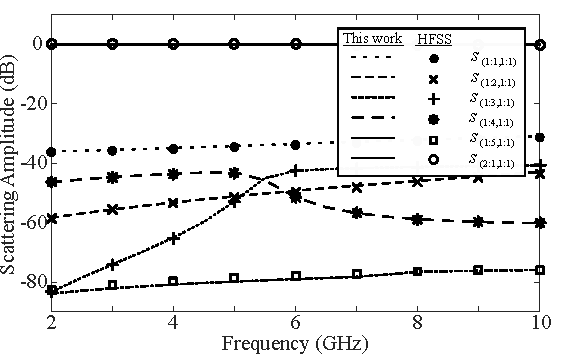
\includegraphics[width=\columnwidth]{spectrum}
\caption{Spectral response of the CPW modal scattering amplitudes given as $s_{(p^r:m^r,p^i:m^i)}$ and compared to HFSS results. }
\label{fig:Scattering}
\end{figure}

A linear analysis is conducted with first order curl-conforming basis functions to ensure proper simulations setup. The choice of the basis order is motivated by the high mesh density within the BST film, principally imposed by its thickness. The mesh is composed of 67,173 tetrahedra, 34,285 in the LAO substrate, 13,105 in the BST film and the remaining 19,783 in the vacuum region. Five modes on each port have been retained during the assembly of system \eqref{eq:FEsys} which has led to 74,208 unknowns, a relatively high number, considering the electrical size of the analysed model. Electrically small geometries and high permittivities cause a small problem to become numerically large in order to accurately approximate the abrupt field variations. The scattering parameters  over the frequency range $[2,10]$~GHz are reported in Fig.~\ref{fig:Scattering}. In particular, these show that the overall crosstalk between lower order modes and impinging fundamental mode is below -40~dB all over the range. Fig.~\ref{fig:fields} shows the electric field distributions when the coplanar ($1^\text{st}$), stripline-like ($2^\text{nd}$) and the microstrip-like ($3^\text{rd}$)  modes are feeding $\Gamma^1_\text{WG}$ and propagating through the CPW at 6~GHz. A decay in fields strength can be appreciated for the higher order modes, these having a high attenuation constant.
%
\begin{figure*}[t!]
\centering
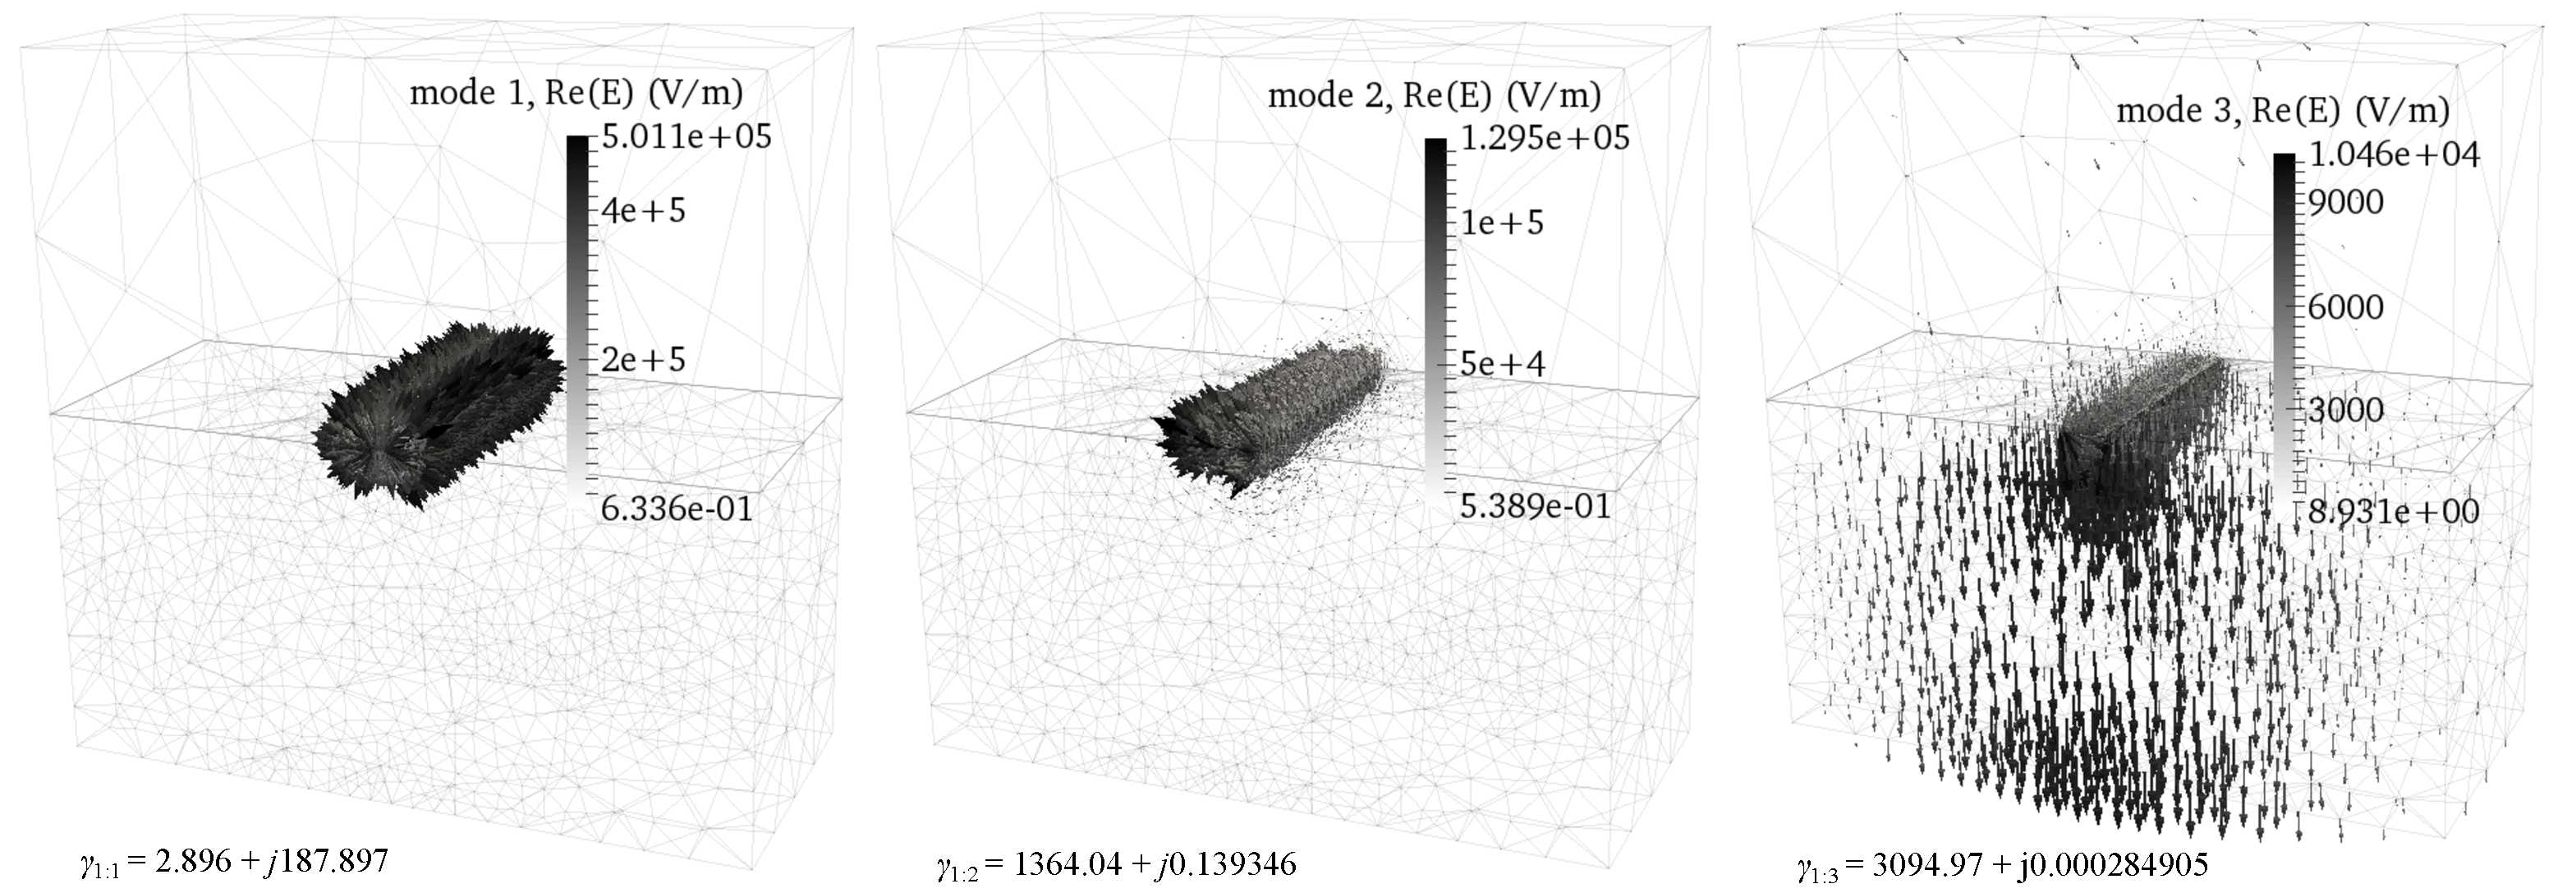
\includegraphics[width=\textwidth]{fields}
\caption{Electric field distributions at 6~GHz within $\Omega$ when the first, coplanar, mode (left), the second, stripline-like, mode (center) and the third, microstrip-like, mode (right) is feeding the CPW through $\Gamma^1_\text{WG}$ with 1 watt of power. }
\label{fig:fields}
\end{figure*}


A first nonlinear analysis is conducted increasing progressively the mesh size, with particular attention to the mesh in the BST, until the power delivered to the third harmonic from an impinging 1~W coplanar mode at 2~GHz converges. Only harmonic orders 1 and 3 ($N=3$) have been kept in these runs. In fact, the nonlinear functional of \eqref{eq:Kerr}, a second order polynomial, is such that odd harmonics do not couple to even ones within the BST, hence no even harmonics can be generated from the impinging fundamental, odd, harmonic. Furthermore, the harmonic expansion of the permittivity will only comprehend the constant term and even harmonics up to $2N$. Here and in the following, the restrictions \mbox{$n=1,3,\ldots,N$} and \mbox{$g=0,2,\ldots,2N$} on the harmonic expansions are employed. Fig.~\ref{fig:convergence} shows that convergence is achieved with almost $10^5$ unknowns. The last mesh refinement, employed for the following analyses, has led to 235,432 unknowns and the total memory and time requirements for the assembly and solve in three iterations were, respectively, 4,698~MB and 229~s.
%
\begin{figure}[ht!]
\centering
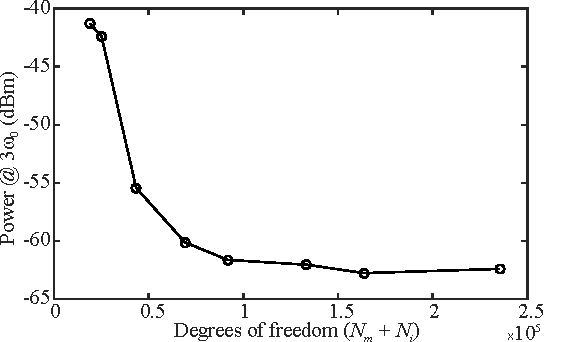
\includegraphics[width=\columnwidth]{convergence}
\caption{Third harmonic spurious power convergence behavior with the number of unknowns of the HBFE system ($N=3$).}
\label{fig:convergence}
\end{figure}

Fig.~\ref{fig:harm_conv} shows the relative error analysis on the fundamental, third and fifth harmonics while progressively increasing $N$ from 3 to 7. The error is defined as
%
\begin{equation*}
\text{Error}(n,N) = \frac{\left| |{s^n_{(2:1,1:1)}}|^{N} - |{s^n_{(2:1,1:1)}}|^{N-2}\right|}{|{s^n_{(2:1,1:1)}}|^{N}}
\end{equation*}
%
\noindent where $n$ is the monitored harmonic number. Increasing the harmonic order of the HBFE system evidently improves the lower order harmonics accuracy. However, it is worth noticing that the system with $N=3$ is accurate up to the sixth decimal place. 
%
\begin{figure}[ht!]
\centering
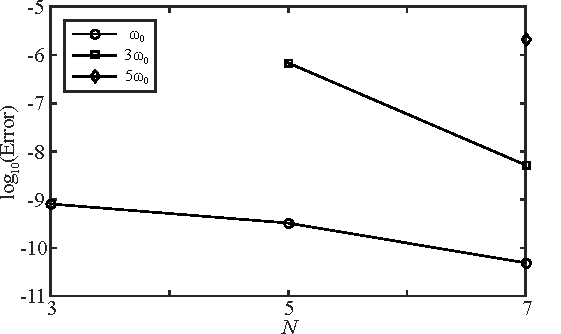
\includegraphics[width=\columnwidth]{harm_conv}
\caption{Relative error on the first, third and fifth harmonics while increasing the HBFE system order.}
\label{fig:harm_conv}
\end{figure}

Finally, the nonlinear analysis is conducted with $N=3$ for different impinging powers on $\Gamma^1_\text{WG}$ at 2~GHz: $\rho^i_{1:1} \equiv$ $10^{-3}$, $10^{-2}$,  $10^{-1}$ and $1$.  
The results of the power sweep are shown in Fig. \ref{fig:third_harm}, denoting good agreements with measurements performed by Mateu \textit{et al.} \cite{mateu2006measurements}. There is almost 2.5~dB overestimation by HBFE predictions with respect to the reported linear interpolation of the third order signal measurements.
%
\begin{figure}[ht!]
\centering
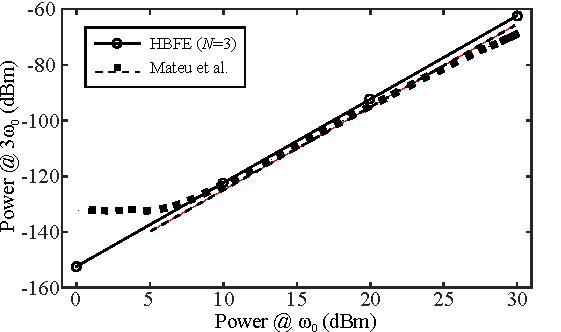
\includegraphics[width=\columnwidth]{third_harm}
\caption{Third harmonic spurious power computed with the HBFE method. Comparisons are with measurements reported in\cite{mateu2006measurements}.}
\label{fig:third_harm}
\end{figure}
%

\section{Conclusion}
A harmonic balance approach to the finite element prediction of spurious harmonics engendered in microwave devices from nonlinear passive dielectrics, for instance ferroelectric materials as the Barium-Strontium-Titanate oxides, has been presented. Simulation results have been discussed in terms of their accuracy and compared to reported measurements.

\section{Acknowledgment}
The authors would like to thank Prof. J. Mateu for providing further details on the measured samples.

\bibliographystyle{IEEEtran}
\bibliography{IEEEabrv,MTT_HBFE}


\end{document}